% Options for packages loaded elsewhere
% Options for packages loaded elsewhere
\PassOptionsToPackage{unicode}{hyperref}
\PassOptionsToPackage{hyphens}{url}
%
\documentclass[
  ignorenonframetext,
  aspectratio=169,
]{beamer}
\newif\ifbibliography
\usepackage{pgfpages}
\setbeamertemplate{caption}[numbered]
\setbeamertemplate{caption label separator}{: }
\setbeamercolor{caption name}{fg=normal text.fg}
\beamertemplatenavigationsymbolsempty
% remove section numbering
\setbeamertemplate{part page}{
  \centering
  \begin{beamercolorbox}[sep=16pt,center]{part title}
    \usebeamerfont{part title}\insertpart\par
  \end{beamercolorbox}
}
\setbeamertemplate{section page}{
  \centering
  \begin{beamercolorbox}[sep=12pt,center]{section title}
    \usebeamerfont{section title}\insertsection\par
  \end{beamercolorbox}
}
\setbeamertemplate{subsection page}{
  \centering
  \begin{beamercolorbox}[sep=8pt,center]{subsection title}
    \usebeamerfont{subsection title}\insertsubsection\par
  \end{beamercolorbox}
}
% Prevent slide breaks in the middle of a paragraph
\widowpenalties 1 10000
\raggedbottom
\AtBeginPart{
  \frame{\partpage}
}
\AtBeginSection{
  \ifbibliography
  \else
    \frame{\sectionpage}
  \fi
}
\AtBeginSubsection{
  \frame{\subsectionpage}
}
\usepackage{iftex}
\ifPDFTeX
  \usepackage[T1]{fontenc}
  \usepackage[utf8]{inputenc}
  \usepackage{textcomp} % provide euro and other symbols
\else % if luatex or xetex
  \usepackage{unicode-math} % this also loads fontspec
  \defaultfontfeatures{Scale=MatchLowercase}
  \defaultfontfeatures[\rmfamily]{Ligatures=TeX,Scale=1}
\fi
\usepackage{lmodern}

\usetheme[]{default}
\ifPDFTeX\else
  % xetex/luatex font selection
\fi
% Use upquote if available, for straight quotes in verbatim environments
\IfFileExists{upquote.sty}{\usepackage{upquote}}{}
\IfFileExists{microtype.sty}{% use microtype if available
  \usepackage[]{microtype}
  \UseMicrotypeSet[protrusion]{basicmath} % disable protrusion for tt fonts
}{}
\makeatletter
\@ifundefined{KOMAClassName}{% if non-KOMA class
  \IfFileExists{parskip.sty}{%
    \usepackage{parskip}
  }{% else
    \setlength{\parindent}{0pt}
    \setlength{\parskip}{6pt plus 2pt minus 1pt}}
}{% if KOMA class
  \KOMAoptions{parskip=half}}
\makeatother


\usepackage{longtable,booktabs,array}
\newcounter{none} % for unnumbered tables
\usepackage{calc} % for calculating minipage widths
\usepackage{caption}
% Make caption package work with longtable
\makeatletter
\def\fnum@table{\tablename~\thetable}
\makeatother
\usepackage{graphicx}
\makeatletter
\newsavebox\pandoc@box
\newcommand*\pandocbounded[1]{% scales image to fit in text height/width
  \sbox\pandoc@box{#1}%
  \Gscale@div\@tempa{\textheight}{\dimexpr\ht\pandoc@box+\dp\pandoc@box\relax}%
  \Gscale@div\@tempb{\linewidth}{\wd\pandoc@box}%
  \ifdim\@tempb\p@<\@tempa\p@\let\@tempa\@tempb\fi% select the smaller of both
  \ifdim\@tempa\p@<\p@\scalebox{\@tempa}{\usebox\pandoc@box}%
  \else\usebox{\pandoc@box}%
  \fi%
}
% Set default figure placement to htbp
\def\fps@figure{htbp}
\makeatother


% definitions for citeproc citations
\NewDocumentCommand\citeproctext{}{}
\NewDocumentCommand\citeproc{mm}{%
  \begingroup\def\citeproctext{#2}\cite{#1}\endgroup}
\makeatletter
 % allow citations to break across lines
 \let\@cite@ofmt\@firstofone
 % avoid brackets around text for \cite:
 \def\@biblabel#1{}
 \def\@cite#1#2{{#1\if@tempswa , #2\fi}}
\makeatother
\newlength{\cslhangindent}
\setlength{\cslhangindent}{1.5em}
\newlength{\csllabelwidth}
\setlength{\csllabelwidth}{3em}
\newenvironment{CSLReferences}[2] % #1 hanging-indent, #2 entry-spacing
 {\begin{list}{}{%
  \setlength{\itemindent}{0pt}
  \setlength{\leftmargin}{0pt}
  \setlength{\parsep}{0pt}
  % turn on hanging indent if param 1 is 1
  \ifodd #1
   \setlength{\leftmargin}{\cslhangindent}
   \setlength{\itemindent}{-1\cslhangindent}
  \fi
  % set entry spacing
  \setlength{\itemsep}{#2\baselineskip}}}
 {\end{list}}
\usepackage{calc}
\newcommand{\CSLBlock}[1]{\hfill\break\parbox[t]{\linewidth}{\strut\ignorespaces#1\strut}}
\newcommand{\CSLLeftMargin}[1]{\parbox[t]{\csllabelwidth}{\strut#1\strut}}
\newcommand{\CSLRightInline}[1]{\parbox[t]{\linewidth - \csllabelwidth}{\strut#1\strut}}
\newcommand{\CSLIndent}[1]{\hspace{\cslhangindent}#1}



\setlength{\emergencystretch}{3em} % prevent overfull lines

\providecommand{\tightlist}{%
  \setlength{\itemsep}{0pt}\setlength{\parskip}{0pt}}



 


\usepackage{booktabs}
\usepackage{caption}
\usepackage{longtable}
\usepackage{colortbl}
\usepackage{array}
\usepackage{anyfontsize}
\usepackage{multirow}
\usepackage{float}
\usepackage{tabularray}
\usepackage[normalem]{ulem}
\usepackage{graphicx}
\usepackage{rotating}
\UseTblrLibrary{siunitx}
\NewTableCommand{\tinytableDefineColor}[3]{\definecolor{#1}{#2}{#3}}
\newcommand{\tinytableTabularrayUnderline}[1]{\underline{#1}}
\newcommand{\tinytableTabularrayStrikeout}[1]{\sout{#1}}
\input{preamble.tex}
\makeatletter
\@ifpackageloaded{caption}{}{\usepackage{caption}}
\AtBeginDocument{%
\ifdefined\contentsname
  \renewcommand*\contentsname{Table of contents}
\else
  \newcommand\contentsname{Table of contents}
\fi
\ifdefined\listfigurename
  \renewcommand*\listfigurename{List of Figures}
\else
  \newcommand\listfigurename{List of Figures}
\fi
\ifdefined\listtablename
  \renewcommand*\listtablename{List of Tables}
\else
  \newcommand\listtablename{List of Tables}
\fi
\ifdefined\figurename
  \renewcommand*\figurename{Figure}
\else
  \newcommand\figurename{Figure}
\fi
\ifdefined\tablename
  \renewcommand*\tablename{Table}
\else
  \newcommand\tablename{Table}
\fi
}
\@ifpackageloaded{float}{}{\usepackage{float}}
\floatstyle{ruled}
\@ifundefined{c@chapter}{\newfloat{codelisting}{h}{lop}}{\newfloat{codelisting}{h}{lop}[chapter]}
\floatname{codelisting}{Listing}
\newcommand*\listoflistings{\listof{codelisting}{List of Listings}}
\makeatother
\makeatletter
\makeatother
\makeatletter
\@ifpackageloaded{caption}{}{\usepackage{caption}}
\@ifpackageloaded{subcaption}{}{\usepackage{subcaption}}
\makeatother

\usepackage{bookmark}
\IfFileExists{xurl.sty}{\usepackage{xurl}}{} % add URL line breaks if available
\urlstyle{same}
\hypersetup{
  pdftitle={Socioeconomic impacts of Terrestrial Protected Areas: Evidence from Large-Scale National Surveys in Madagascar},
  pdfauthor={Iriana Razafimahenina\^{}\{1,4\}; Florent Bédécarrats\^{}\{2\}; Ingrid Dallmann\^{}\{3\}; Holimalala Randriamanampisoa\^{}\{4\}},
  hidelinks,
  pdfcreator={LaTeX via pandoc}}


\title{\texorpdfstring{Socioeconomic impacts of Terrestrial Protected
Areas: Evidence from Large-Scale National Surveys in
Madagascar}{Socioeconomic impacts of Terrestrial Protected Areas: Evidence from Large-Scale National Surveys in Madagascar}}
\subtitle{\texorpdfstring{WCRE Conference, Lisbon -- 29 june - 3 july
2026}{WCRE Conference, Lisbon -- 29 june - 3 july 2026}}
\author{\textbf{Iriana Razafimahenina}\(^{1,4}\) \and Florent
Bédécarrats\(^{2}\) \and Ingrid Dallmann\(^{3}\) \and Holimalala
Randriamanampisoa\(^{4}\)}
\date{}
\institute{\(^{1}\)University of Paris Saclay \(\quad\)
\(^{2}\)University Versailles Saint Quentin \(\quad\) \(^{3}\)Agence
Française de Développement \(\quad\) \(^{4}\)University of Antananarivo}

\begin{document}
\frame{\titlepage}


\begin{frame}{To what extent do protected areas (PA) impact household
living conditions?}
\protect\phantomsection\label{to-what-extent-do-protected-areas-pa-impact-household-living-conditions}
\hyperlink{annexe-theory-change}{\beamerbutton{$\triangleright$ Theory of change}}

\begin{itemize}
\item
  \textbf{Economic Opportunities}

  \begin{itemize}
  \tightlist
  \item
    Development of local tourism (Naidoo et al. 2019),
  \item
    Creation of conservation-related jobs (Balietti et al. 2024)
  \item
    Compensation measures (Poudyal et al. 2018)
  \item
    Improved ecosystem services (Xu et al. 2023)
  \end{itemize}
\item
  \textbf{Restrictions and Costs} Restricted access to natural resources
  - gathering, hunting, fishing, medicinal plants (Kandel et al. 2022)
\item
  \textbf{Heterogeneous results} Effects vary across evaluation methods,
  institutional contexts, and geographic locations (Kandel et al. 2022).
\end{itemize}
\end{frame}

\begin{frame}{Madagascar is a relevant study case}
\protect\phantomsection\label{madagascar-is-a-relevant-study-case}
\hyperlink{annexe-evolution-PA}{\beamerbutton{$\triangleright$ Evolution of protected areas}}

\begin{columns}[T]
\begin{column}{0.52\linewidth}
\textbf{Surface of PA and Size of the adjacent population exposed to
them nearly tripled between 2008 and 2021}

\begin{itemize}
\tightlist
\item
  2008: 3,6\% of the territory --- 9\% population lived \textless{} 10
  km of PA
\item
  2021: 10,8\% du territoire --- 28\% population lived \textgreater{} 10
  km of PA
\end{itemize}

\textbf{A vulnerable socio-economic context }

\begin{itemize}
\tightlist
\item
  The world's poorest country based on SDG Indicator 1.1 (Conceição
  2024)\\
\item
  High dependence on natural resources (Llopis et al. 2023)\\
\item
  Weak state capacity (Hanson and Sigman 2021)
\end{itemize}

\vspace{0.1cm}
\end{column}

\begin{column}{0.48\linewidth}
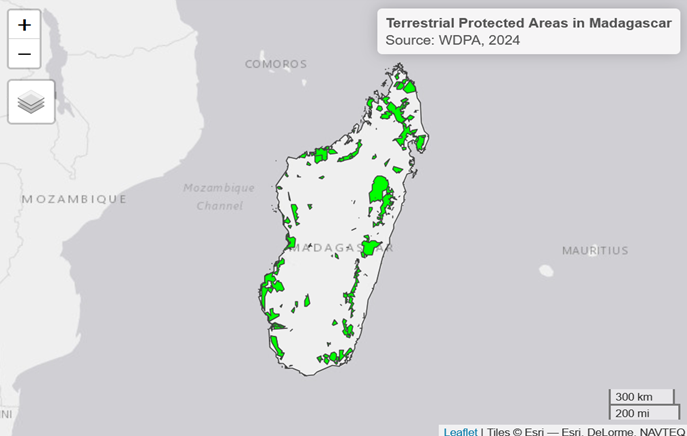
\includegraphics[width=1\linewidth,height=\textheight,keepaspectratio]{images/carte_AP.png}

\tiny Source : Authors
\end{column}
\end{columns}
\end{frame}

\begin{frame}{\textbf{How would household living conditions have evolved
if PA had not been established?}}
\protect\phantomsection\label{how-would-household-living-conditions-have-evolved-if-pa-had-not-been-established}
\begin{columns}[T]

\begin{column}{0.48\linewidth}

\textcolor{vertfonce}{\textbf{Research questions}}

\small
\begin{itemize}
\item \textbf{Q1 :} Do PA worsen the living conditions of local communities?
\item \textbf{Q2 :} Do PA increase inequality among local communities?
\item \textbf{Q3 :} Do the impacts vary by type of PA?
\end{itemize}

\end{column}

\begin{column}{0.04\linewidth}
\end{column}

\begin{column}{0.48\linewidth}

\textcolor{orange}{\textbf{Hypothesis}}

\small
\begin{itemize}
\item \textbf{H1 :} PA in Madagascar may reduce well-being by limiting access to natural resources.
\item \textbf{H2 :} PA may increase inequality through uneven access to benefits.
\item \textbf{H3 :} Impacts are heterogeneous depending on governance and context.
\end{itemize}

\end{column}

\end{columns}
\end{frame}

\begin{frame}{Contribution}
\protect\phantomsection\label{contribution}
\begin{itemize}
\item
  First national-level evaluation of terrestrial PAs in Madagascar (71
  PAs, 2008-2021)
\item
  Robust methodological strategy: matching + DID applied to geolocated
  household survey data
\end{itemize}
\end{frame}

\begin{frame}{The data at the rural level}
\protect\phantomsection\label{the-data-at-the-rural-level}
\hyperlink{annexe-empirical-methodology}{\beamerbutton{$\triangleright$ Summary statistics}}

\begin{table}[ht]
\centering
\vbox{
\resizebox{0.90\textwidth}{!}{ 
\tiny % Force tout le texte du tableau à être très petit
\begin{tabular}{>{\columncolor{vertclair}}p{2.2cm} p{3.4cm} p{4.6cm}}
\toprule
\rowcolor{vertfonce}
\textcolor{white}{\textbf{Role in the analysis}} &
\textcolor{white}{\textbf{Variable names}} &
\textcolor{white}{\textbf{Data source}} \\
\midrule
Treatment variable & Protected Areas & \textit{World Database on Protected Areas} (2025) \\
\midrule
& Wealth index & \textit{DHS/MIS/MICS} (1997, 2008, 2011, 2016, 2018, 2021) \\
\multirow{-2.2}{2.2cm}{Outcome variable} & Zscore of the wealth index & \\
\midrule
& Forest cover rates in 2000 & \textit{Global Forest Change} [Hansen2013] \\
& Population density in 2000 & \textit{WorldPop} [WorldPop2018] \\
& Accessibility in 2000 & \textit{JRC} [Uchida2011] \\
\multirow{-4}{2.2cm}{Matching variables} & Slope and elevation & NASA-SRTM [NASAJPL2020] \\
\midrule
& Sex and age of the head of household & \textit{DHS/MIS/MICS} (1997, 2008, 2011, 2016, 2018, 2021) \\
\multirow{-2.2}{2.2cm}{Control variables} & Drought index (SPEI) & [VicenteSerrano2010] \\
\midrule
Moderating variable & IUCN categories & [DHS/MIS/MICS]\\
\bottomrule
\end{tabular}
}
}
\end{table}
\end{frame}

\begin{frame}{Counterfactual analysis}
\protect\phantomsection\label{counterfactual-analysis}
\begin{columns}[T]
\begin{column}{0.48\linewidth}
\begin{itemize}
\item
  \textbf{Treatment}: Establishment of PA between 2008 and 2021
\item
  \textbf{Treatment group}: Rural Households located in clusters
  \textless{} 10 km of PA created between 2008 and 2021
\item
  \textbf{Control group}: Rural Households located in clusters
  \textgreater{} 10 km of PA created between 2008 and 2021
\item
  \textbf{Excluded group}: Households located in clusters within
  \textless{} 10 km of PA created before 2008 and in urban areas
\end{itemize}

\vspace{0.3cm}
\end{column}

\begin{column}{0.52\linewidth}
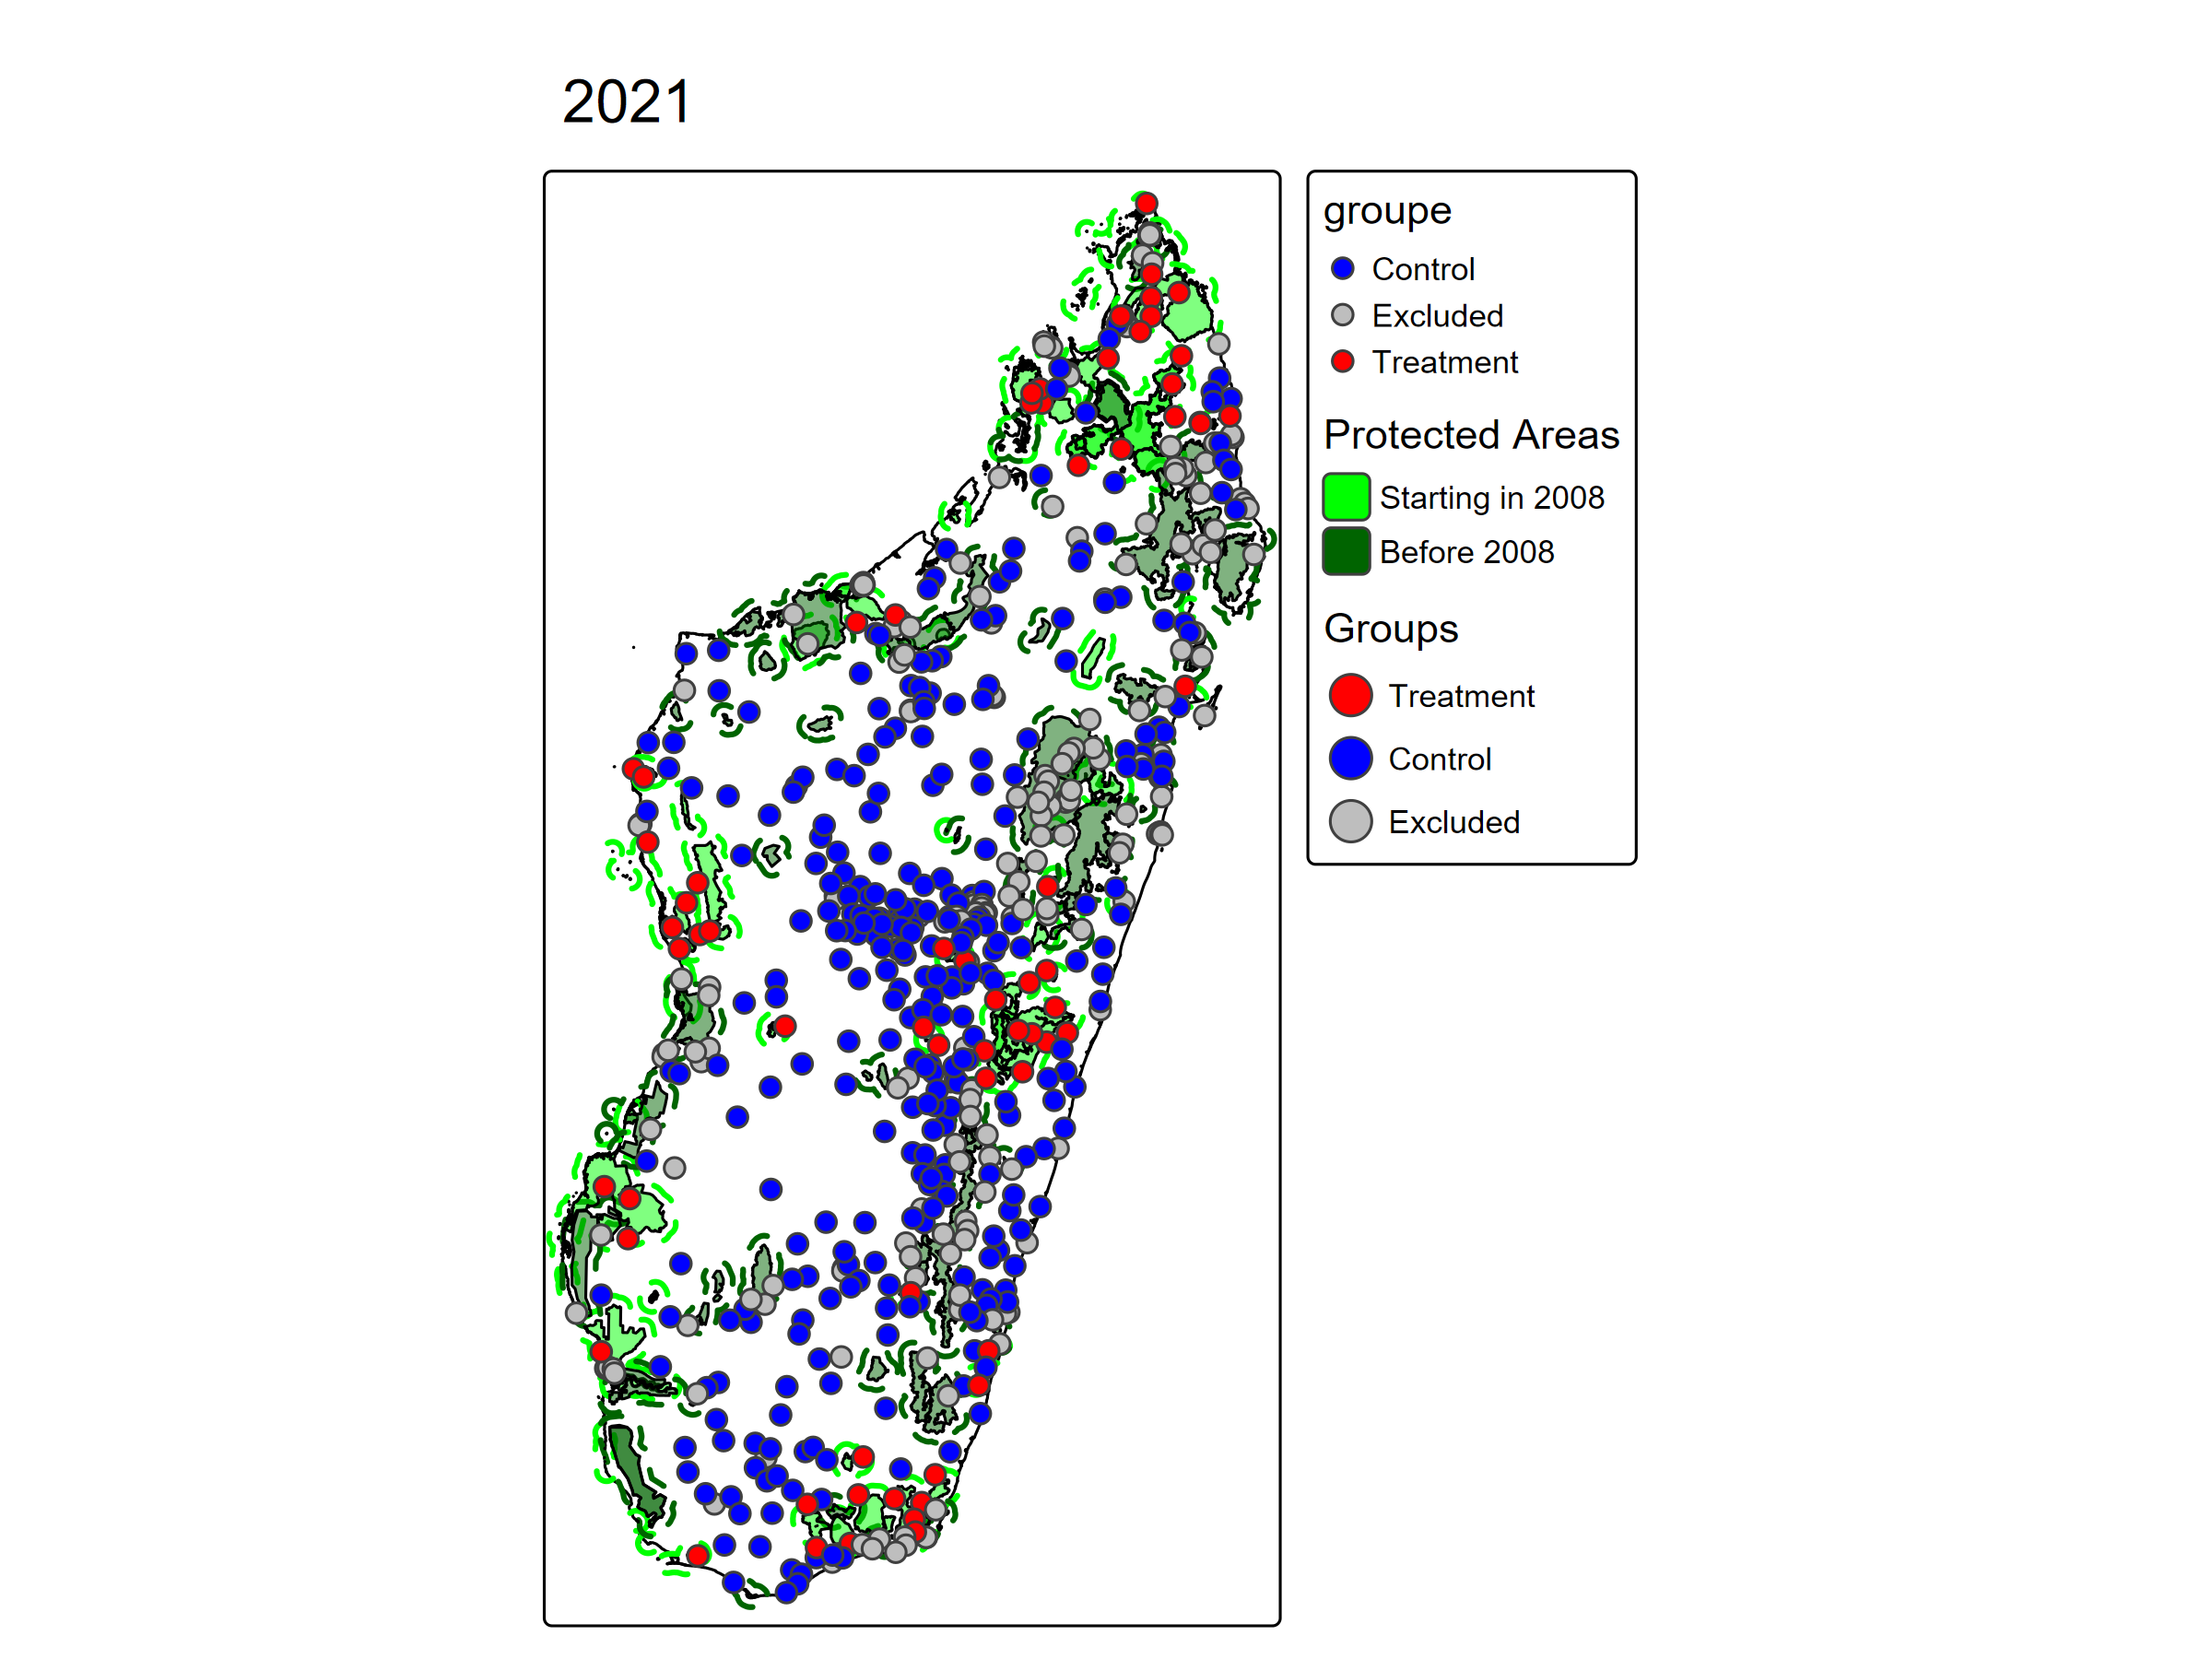
\includegraphics[width=1.1\linewidth,height=\textheight,keepaspectratio]{images/map_2021.png}

\tiny Source: Authors based on DHS, WDPA data
\end{column}
\end{columns}
\end{frame}

\begin{frame}{Estimating the impact of PA on living condition}
\protect\phantomsection\label{estimating-the-impact-of-pa-on-living-condition}
\begin{itemize}
\item
  \textbf{Genetic matching}: To compare observable characteristics
  between the treatment group and the control group (Diamond and Sekhon
  2013)
  \hyperlink{annexe-matching}{\beamerbutton{$\triangleright$ Matching }}
\item
  \textbf{Difference-in-difference (DID)}
\end{itemize}

\small

\[
Y_{ict} = \alpha + \delta \cdot (\mathrm{Treatment}_c \times \mathrm{Post}_t) + X_{ict}' \theta + \mu_c + \lambda_t + \varepsilon_{ict}
\]

\fontsize{4pt}{5pt}\selectfont
\setlength{\itemsep}{0pt}
\setlength{\parskip}{0pt}
\setlength{\parsep}{0pt}
\setlength{\topsep}{0pt}
\begin{itemize}
  \item $Y_{ict}$: wealth index (hh $i$, cluster $c$, year $t$)
  \item $\delta$: DID effect (PA → welfare)
  \item $\text{Treat}_c \times \text{Post}_t$: DID term
  \item $\mu_c,\lambda_t$: cluster fixed effects
  \item $X_{ict}$: controls (age/sex of the head of household, SPEI, accessibility, population density, forest cover rate, slope, altitude)
\end{itemize}
\end{frame}

\begin{frame}{PA impact on the household wealth index}
\protect\phantomsection\label{pa-impact-on-the-household-wealth-index}
\hyperlink{annexe-result-h1}{\beamerbutton{$\triangleright$ Impact on well-being: Event study with 2 year bins}}

\begin{columns}[T]
\begin{column}{0.52\linewidth}
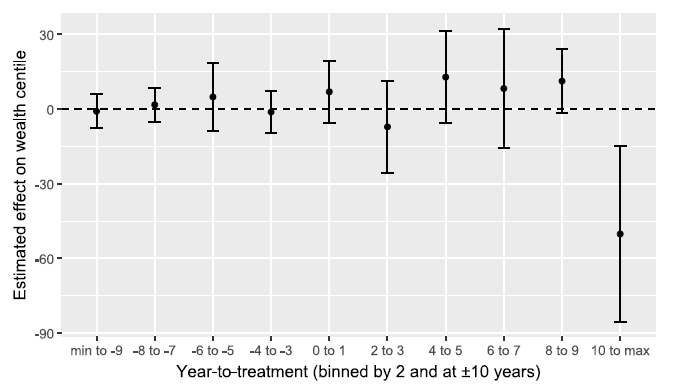
\includegraphics[width=1\linewidth,height=\textheight,keepaspectratio]{images/result_H1.png}

\vspace{0.1cm}
\end{column}

\begin{column}{0.48\linewidth}
\begin{itemize}
\item
  No significant effect of PA on the household wealth index
\item
  Losses associated with restrictions offset by gains elsewhere -
  (conservation related job, economic activities)
\item
  Offsetting effects may neutralize the overall impact in the short and
  medium term
\end{itemize}
\end{column}
\end{columns}
\end{frame}

\begin{frame}{PA impact on the household wealth index inequalities}
\protect\phantomsection\label{pa-impact-on-the-household-wealth-index-inequalities}
\hyperlink{annexe-result-h2}{\beamerbutton{$\triangleright$ "Impact on inequalities: Event-study with 2-year bins}}

\begin{columns}[T]
\begin{column}{0.52\linewidth}
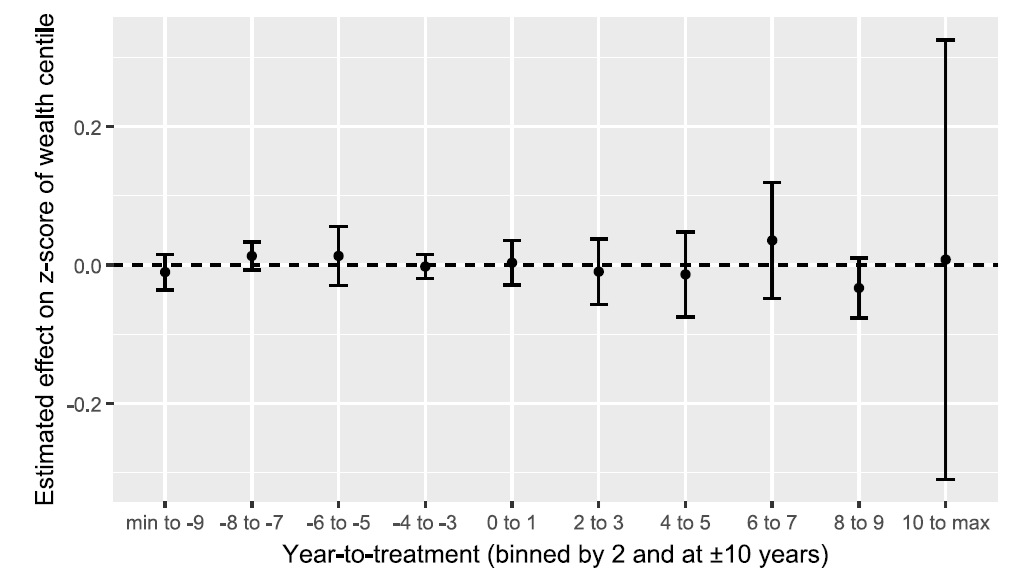
\includegraphics[width=1\linewidth,height=\textheight,keepaspectratio]{images/result_H2.png}

\vspace{0.1cm}
\end{column}

\begin{column}{0.48\linewidth}
\begin{itemize}
\tightlist
\item
  No significant effect of PA creation on a wealth inequality
\item
  Inequality is mainly driven by sociodemographic and climate related
  factors:

  \begin{itemize}
  \tightlist
  \item
    Droughts impoverish vulnerable households
  \item
    Female headed households tend to have lower wealth
  \item
    Household headed by other people tend to be wealthier
  \end{itemize}
\end{itemize}
\end{column}
\end{columns}
\end{frame}

\begin{frame}{Heterogeneity: Which PA Harm Most?}
\protect\phantomsection\label{heterogeneity-which-pa-harm-most}
\hyperlink{annexe-result-h3}{\beamerbutton{$\triangleright$ "Heterogeneity of impact on well-being}}

\begin{columns}[T]
\begin{column}{0.52\linewidth}
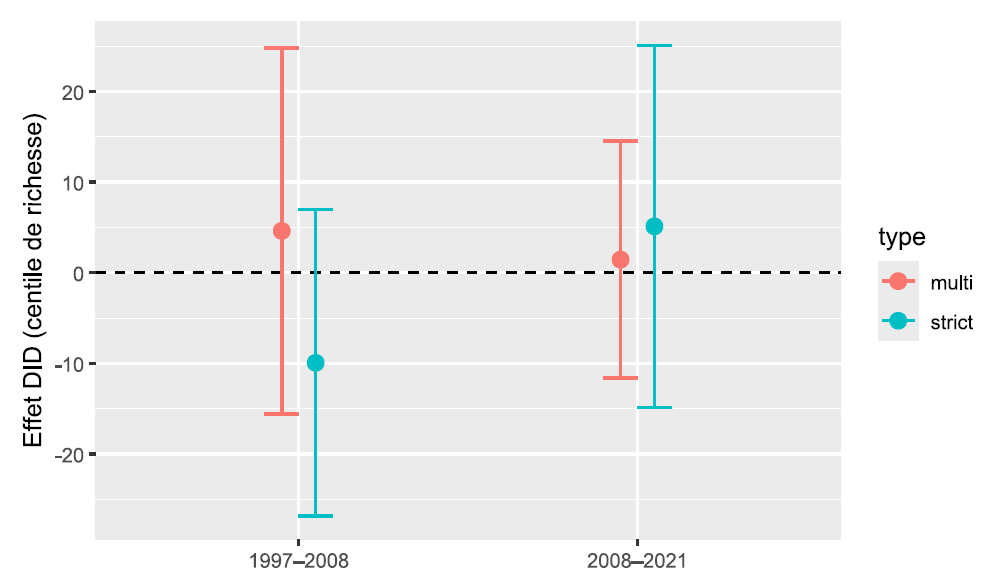
\includegraphics[width=1\linewidth,height=\textheight,keepaspectratio]{images/result_H3.png}

\vspace{0.1cm}
\end{column}

\begin{column}{0.48\linewidth}
\begin{itemize}
\tightlist
\item
  No significant effect of PA governance categories on the household
  wealth index
\item
  Results highlights the limits of formal governance categories to
  explain the socioeconomic outcomes of PA
\end{itemize}
\end{column}
\end{columns}
\end{frame}

\begin{frame}{Conclusions}
\protect\phantomsection\label{conclusions}
\begin{itemize}
\item
  No significant average effect on the standards of conditions - losses
  associated with restrictions appear to be offset by adaptation
  mechanisms and local opportunities
\item
  No significant effect on inequality - the main determinants remain
  climate shocks and sociodemographic characteristics
\item
  No differentiated effect based on governance type - formal categories
  alone do not explain socioeconomic outcomes
\item
  Across distance thresholds (5km/15km) and alternative outcome
  variables , results consistently show \textbf{no significant effect of
  PA on household welfare}
\end{itemize}

\textbf{Next steps}:

Understanding the determinants of these impacts: protected area
governance and management modalities
\end{frame}

\begin{frame}{}
\protect\phantomsection\label{section}
\vfill

\begin{center}

{\Large \textbf{Thank you for your attention}}

\vspace{1cm}

{\normalsize \textit{Questions \& Discussion}}

\vspace{1.5cm}

{\small \textbf{Contact:} iriana\_ny\_aina.razafimahenina@ird.fr}

\end{center}

\vfill
\end{frame}

\begin{frame}[allowframebreaks]{References}
\protect\phantomsection\label{references}
\footnotesize

\protect\phantomsection\label{refs}
\begin{CSLReferences}{1}{1}
\bibitem[\citeproctext]{ref-baliettiLaborMarketImpacts2024}
Balietti, Anca, Sreeja Jaiswal, and Daniel Schäffer. 2024. {``Labor
Market Impacts of Eco-Development Initiatives in Protected Areas.''}
\emph{Journal of Environmental Economics and Management} 128 (November):
103070. \url{https://doi.org/10.1016/j.jeem.2024.103070}.

\bibitem[\citeproctext]{ref-Conceicao2024}
Conceição, Pedro, ed. 2024. \emph{Breaking the Gridlock: {Reimagining}
Cooperation in a {Polarized} World}. Human {Development} {Report},
2023/2024. UNDP.

\bibitem[\citeproctext]{ref-Diamond2013}
Diamond, Alexis, and Jasjeet S. Sekhon. 2013. {``Genetic {Matching} for
{Estimating} {Causal} {Effects}: {A} {General} {Multivariate} {Matching}
{Method} for {Achieving} {Balance} in {Observational} {Studies}.''}
\emph{Review of Economics and Statistics} 95 (3): 932--45.
\url{https://doi.org/10.1162/REST_a_00318}.

\bibitem[\citeproctext]{ref-Hanson2021}
Hanson, Jonathan K., and Rachel Sigman. 2021. {``Leviathan's {Latent}
{Dimensions}: {Measuring} {State} {Capacity} for {Comparative}
{Political} {Research}.''} \emph{The Journal of Politics} 83 (4):
1495--510. \url{https://doi.org/10.1086/715066}.

\bibitem[\citeproctext]{ref-Kandel2022}
Kandel, Pratikshya, Ram Pandit, Benedict White, and Maksym Polyakov.
2022. {``Do Protected Areas Increase Household Income? {Evidence} from a
{Meta}-{Analysis}.''} \emph{World Development} 159 (November): 106024.
\url{https://doi.org/10.1016/j.worlddev.2022.106024}.

\bibitem[\citeproctext]{ref-Llopis2023}
Llopis, Jorge C., Clara L. Diebold, Flurina Schneider, et al. 2023.
{``Mixed Impacts of Protected Areas and a Cash Crop Boom on Human
Well‐being in {North}‐{Eastern} {Madagascar}.''} \emph{People and
Nature} 5 (6): 1786--803. \url{https://doi.org/10.1002/pan3.10377}.

\bibitem[\citeproctext]{ref-Naidoo2019}
Naidoo, R., D. Gerkey, D. Hole, et al. 2019. {``Evaluating the Impacts
of Protected Areas on Human Well-Being Across the Developing World.''}
\emph{Science Advances} 5 (4): eaav3006.
\url{https://doi.org/10.1126/sciadv.aav3006}.

\bibitem[\citeproctext]{ref-Poudyal2018}
Poudyal, Mahesh, Julia PG Jones, O. Sarobidy Rakotonarivo, et al. 2018.
{``Who Bears the Cost of Forest Conservation?''} \emph{PeerJ} 6: e5106.
\url{https://doi.org/10.7717/peerj.5106}.

\bibitem[\citeproctext]{ref-Xu2023}
Xu, Shang, H. Allen Klaiber, and Daniela A. Miteva. 2023. {``Impacts of
Forest Conservation on Local Agricultural Labor Supply: {Evidence} from
the {Indonesian} Forest Moratorium.''} \emph{American Journal of
Agricultural Economics} 105 (3): 940--65.
\url{https://doi.org/10.1111/ajae.12344}.

\end{CSLReferences}
\end{frame}

\section*{Appendix}\label{appendix}
\addcontentsline{toc}{section}{Appendix}

\begin{frame}{Appendix}
\appendix
\end{frame}

\begin{frame}{Theory of Change}
\protect\phantomsection\label{theory-of-change}
\hypertarget{annexe-theory-change}{}

\begin{figure}
  \centering
  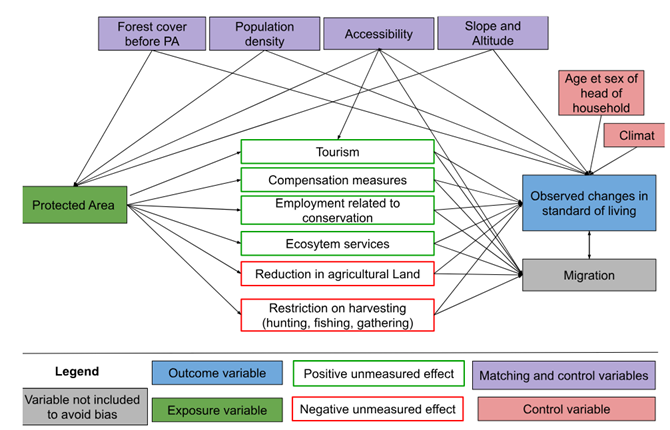
\includegraphics[width=0.95\textwidth, height=0.75\textheight, keepaspectratio]{images/theory_of_change.png}
  \caption{\tiny Logic diagram of the theory of change}
  \tiny{\textit{Source : Auteurs}}
\end{figure}

\hyperlink{slide-context}{\beamerbutton{$\leftarrow$ Back}}
\end{frame}

\begin{frame}{Evolution of protected areas}
\protect\phantomsection\label{evolution-of-protected-areas}
\hypertarget{annexe-evolution-PA}{}

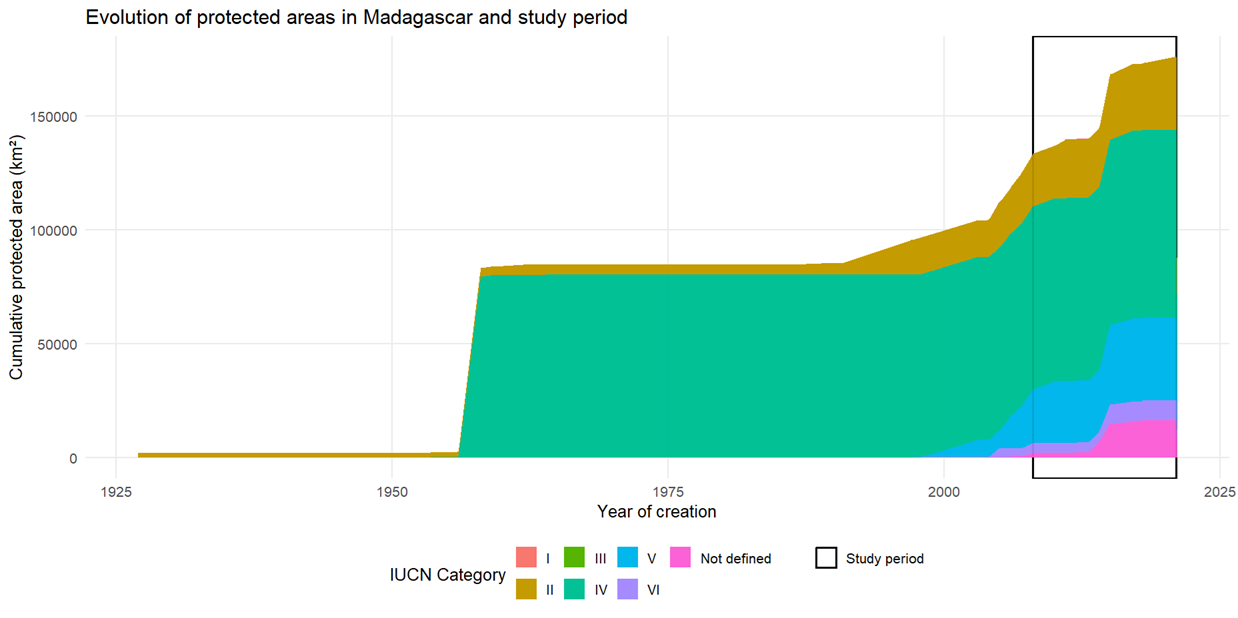
\includegraphics[width=0.9\linewidth,height=\textheight,keepaspectratio]{images/evo_pa.png}

\hyperlink{slide-context}{\beamerbutton{$\leftarrow$ Back}}
\end{frame}

\begin{frame}{Summary statistics: Distribution of the rural wealth
index}
\protect\phantomsection\label{summary-statistics-distribution-of-the-rural-wealth-index}
\hypertarget{annexe-empirical-methodology}{}

\begin{figure}[H]

\centering{

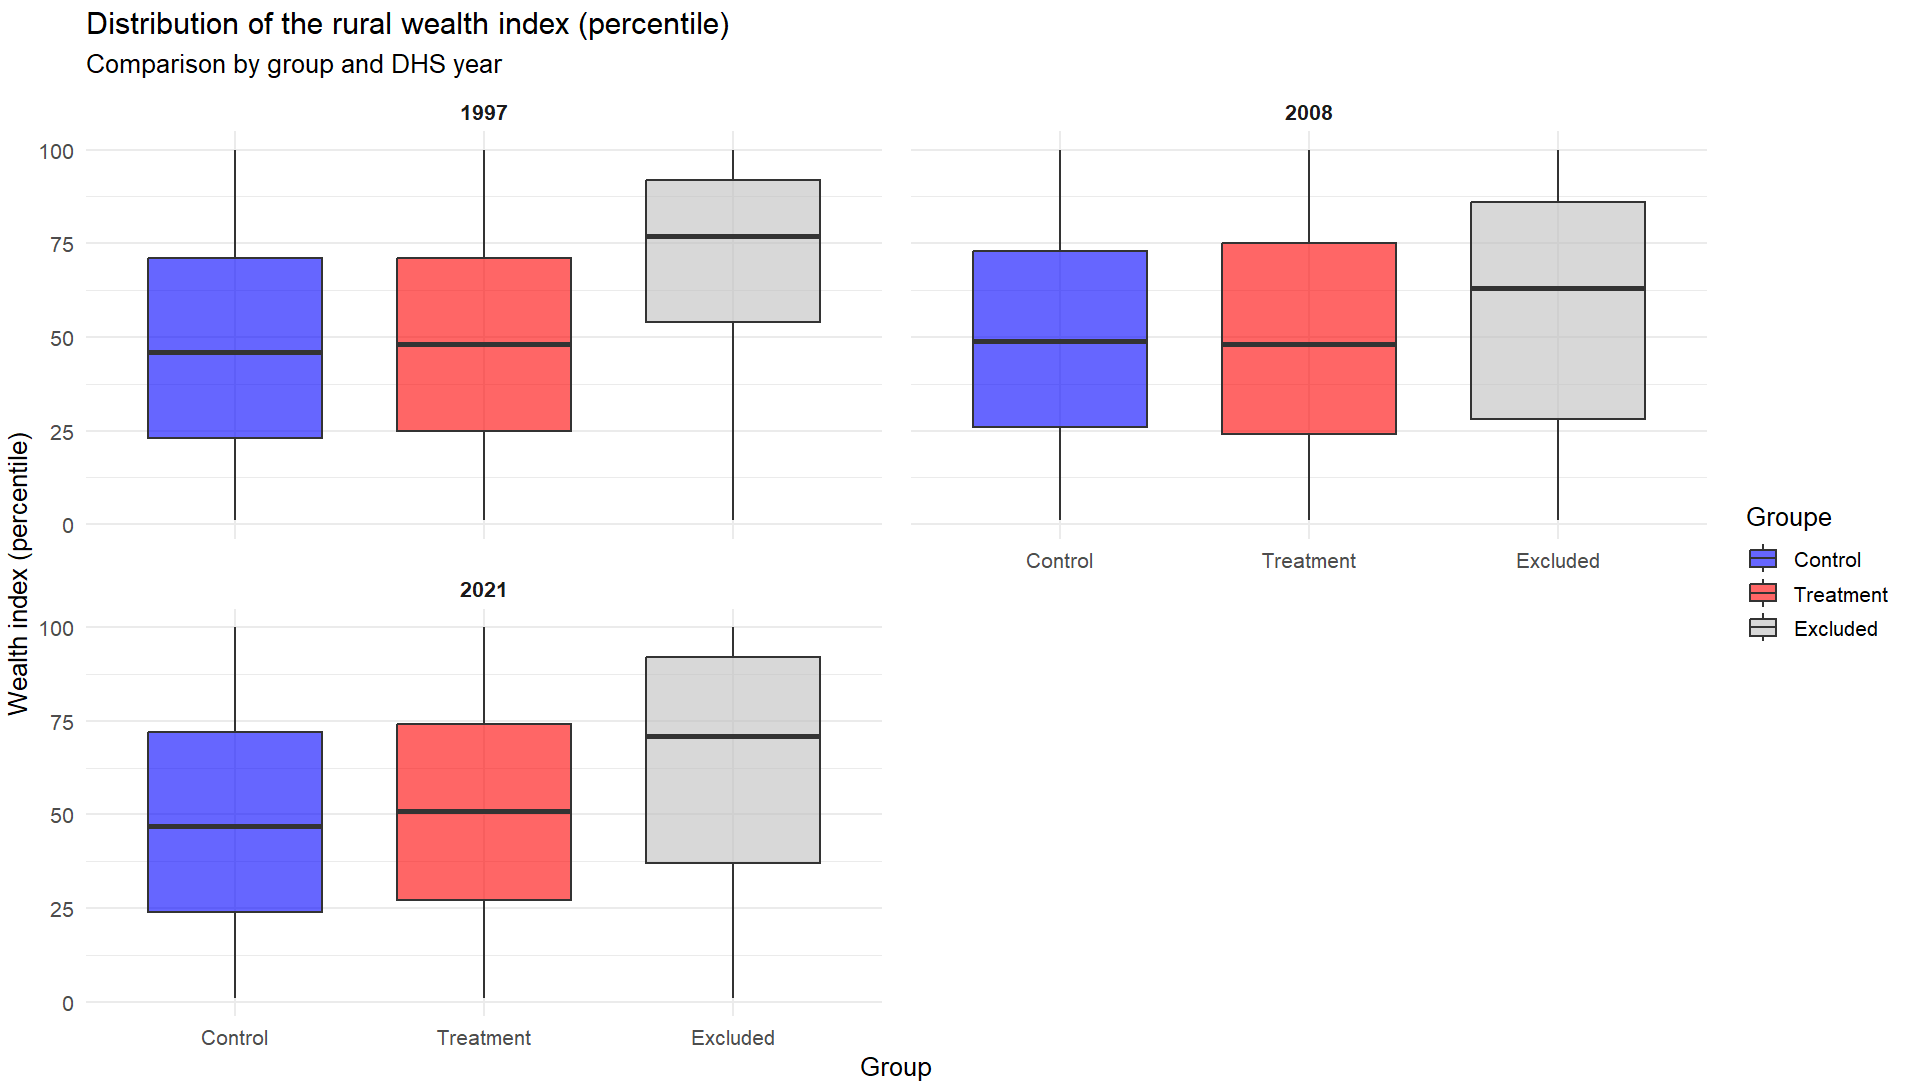
\includegraphics[width=0.8\linewidth,height=\textheight,keepaspectratio]{images/distr_wi.png}

}

\caption{\label{fig-distr-wi}Distribution of the rural wealth index
(percentile)}

\end{figure}%

\emph{Source: Authors}

\hyperlink{slide-empirical-methodology}{\beamerbutton{$\leftarrow$ Back}}
\end{frame}

\begin{frame}{Summary statistics: Distribution of the Z-score of the
rural wealth index}
\protect\phantomsection\label{summary-statistics-distribution-of-the-z-score-of-the-rural-wealth-index}
\begin{figure}[H]

\centering{

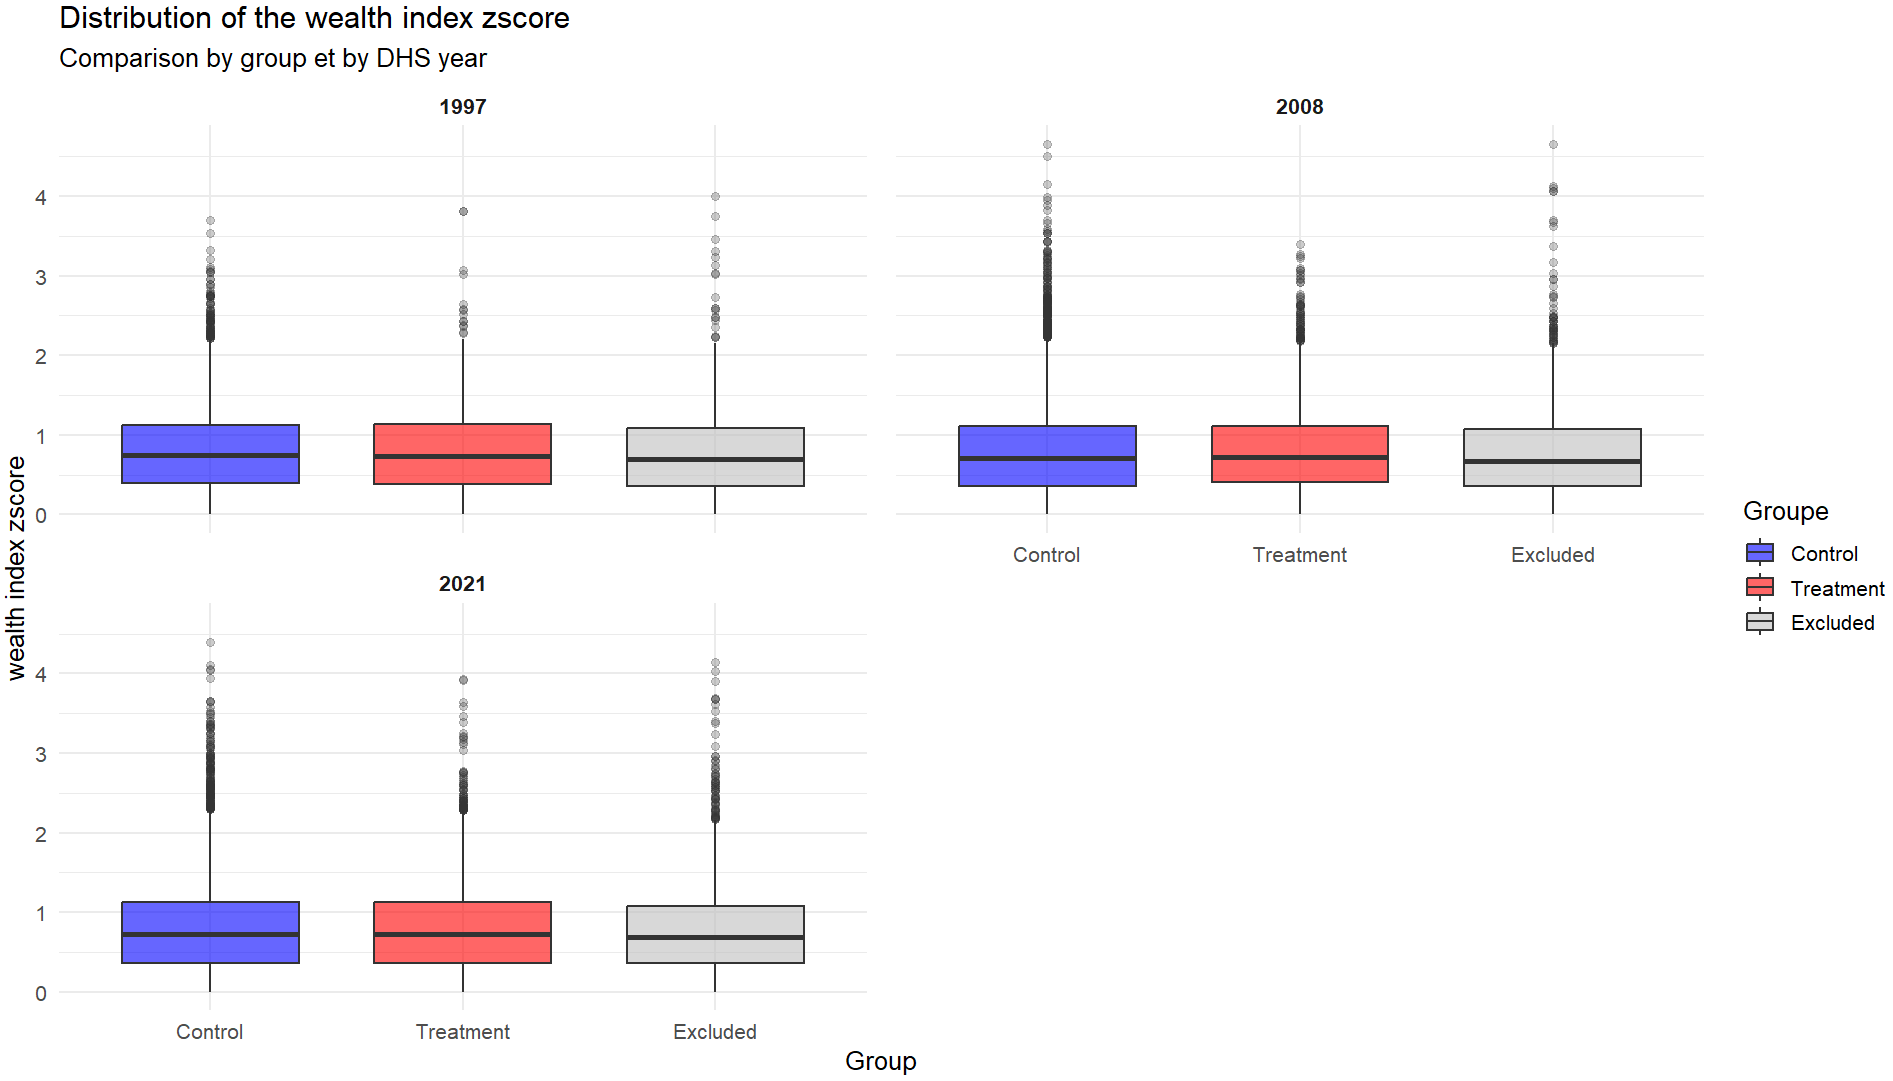
\includegraphics[width=0.8\linewidth,height=\textheight,keepaspectratio]{images/distr_zs.png}

}

\caption{\label{fig-distr-zs}Distribution of the Z-score of the rural
wealth index (percentile)}

\end{figure}%

\emph{Source: Authors}

\hyperlink{slide-empirical-methodology}{\beamerbutton{$\leftarrow$ Back}}
\end{frame}

\begin{frame}[shrink]{Descriptive statistics}
\protect\phantomsection\label{descriptive-statistics}
\hyperlink{annexe-empirical-methodology}{\beamerbutton{$\triangleright$ Descriptive statistics}}

\begin{table}

\caption{\label{tbl-gt-desc-AP}Descriptive statistics for protected
areas created before 2008 and from 2021}

\centering{

\fontsize{5.0pt}{6.0pt}\selectfont
\begin{tabular*}{1\linewidth}{@{\extracolsep{\fill}}lrrrrrlrl}
\toprule
periode & n & mean & sd & median & min & aire\_min & max & aire\_max \\ 
\midrule\addlinespace[2.5pt]
From 2008 & 84.00 & 574.17 & 1,017.13 & 205.27 & 0.28 & Nosy Antsoha & 5,688.62 & Complexe des  AP Ambohimirahavavy Marivorahona \\ 
Before 2008 & 60.00 & 2,087.61 & 10,070.25 & 247.69 & 0.05 & Parc de Tsarasaotra & 78,139.00 & Ambatovaky \\ 
\bottomrule
\end{tabular*}

}

\end{table}%
\end{frame}

\begin{frame}{Matching \{.unnumbered .shrink\} (1/2)}
\protect\phantomsection\label{matching-.unnumbered-.shrink-12}
\hypertarget{annexe-evolution-PA}{}

\small

\begin{table}

\caption{\label{tbl-balance-long-2008}Standardized Mean Difference of
the Year 2008 and 2021}

\centering{

\caption*{
{\fontsize{20}{25}\selectfont  Covariates balance before and after matching\fontsize{5}{7}\selectfont }
} 
\fontsize{5.0pt}{6.0pt}\selectfont
\begin{tabular*}{1\linewidth}{@{\extracolsep{\fill}}lcccc}
\toprule
 & \multicolumn{2}{c}{2008} & \multicolumn{2}{c}{2021} \\ 
\cmidrule(lr){2-3} \cmidrule(lr){4-5}
Variable & Before matching & After matching & Before matching & After matching \\ 
\midrule\addlinespace[2.5pt]
Elevation (m) & 0.568 & 0.056 & 0.433 & 0.092 \\ 
Population density in 2000 (km\texttwosuperior) & 0.976 & 0.050 & 1.172 & 0.086 \\ 
Slope (\%) & 0.105 & 0.018 & 0.150 & 0.012 \\ 
Accessibility in 2000 (min) & 0.365 & 0.018 & 0.379 & 0.047 \\ 
Forest cover rates in 2000 (\%) & 0.729 & 0.007 & 0.925 & 0.101 \\ 
\bottomrule
\end{tabular*}

}

\end{table}%

\hyperlink{slide-context}{\beamerbutton{$\leftarrow$ Back}}
\end{frame}

\begin{frame}{Matching}
\protect\phantomsection\label{matching}
\begin{columns}[T]
\begin{column}{0.5\linewidth}
\begin{block}{Before 2008}
\protect\phantomsection\label{before-2008}
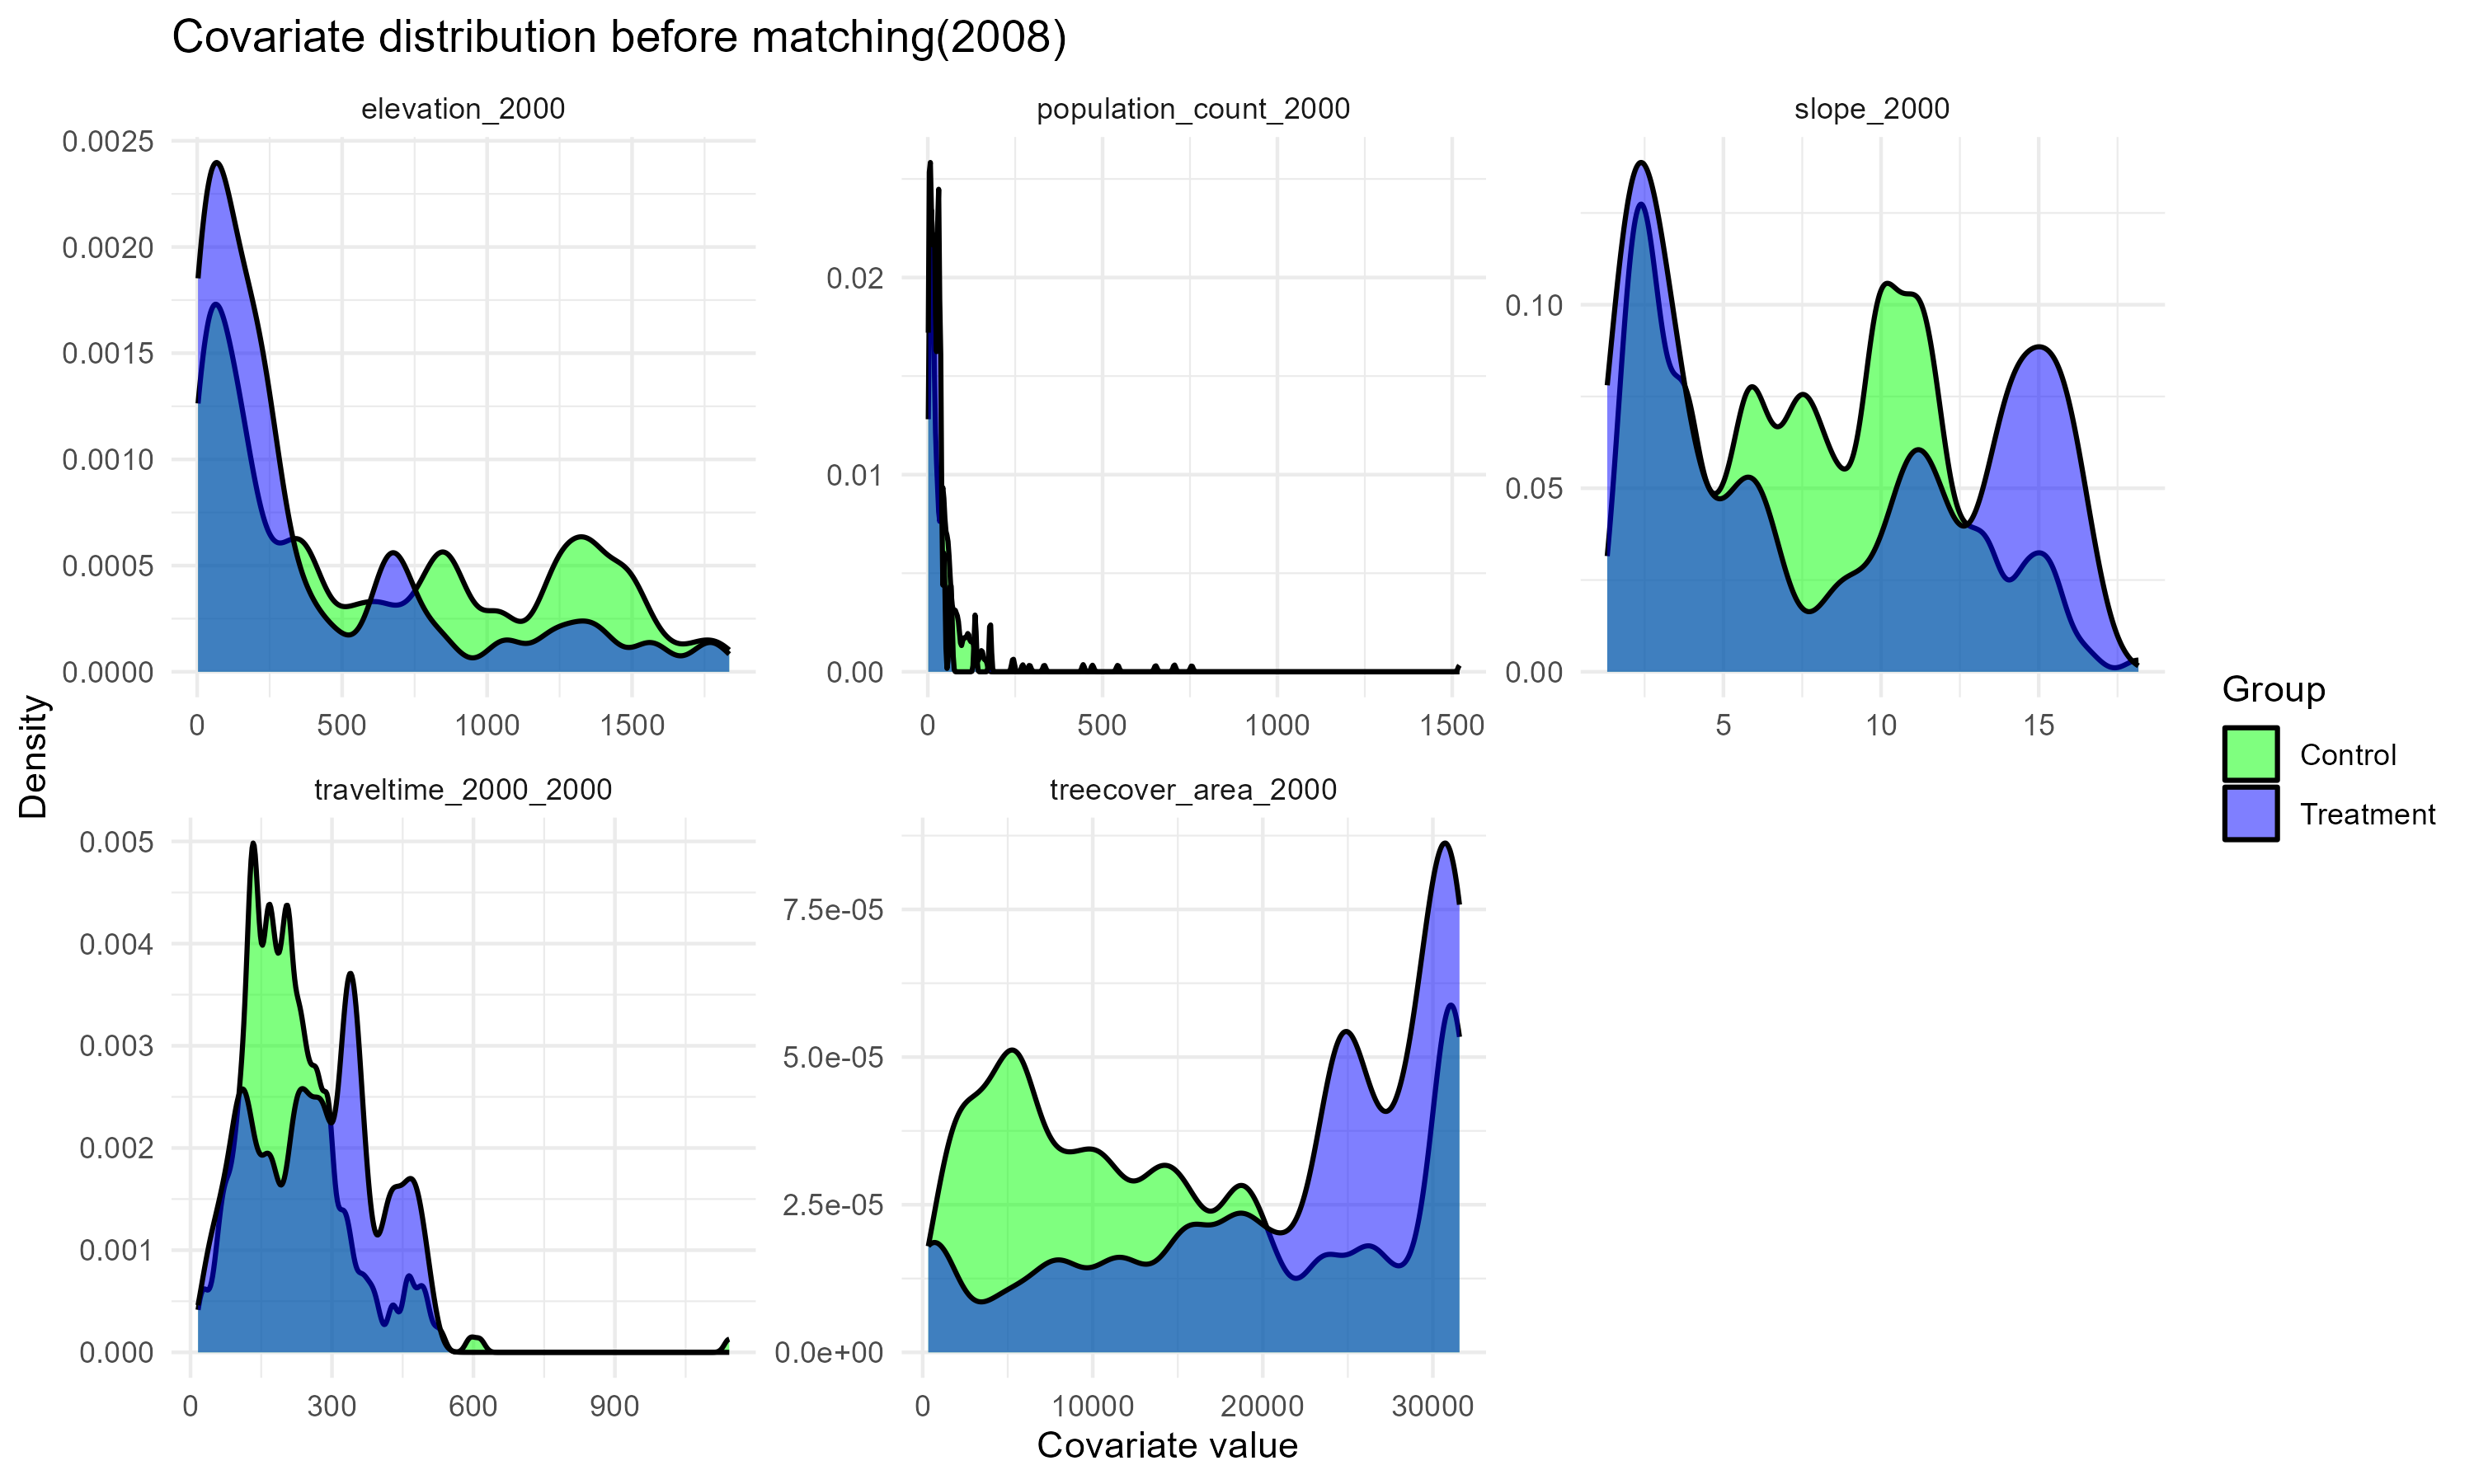
\includegraphics[width=1\linewidth,height=\textheight,keepaspectratio]{images/density_before_2008.png}
\end{block}
\end{column}

\begin{column}{0.5\linewidth}
\begin{block}{After matching 2008}
\protect\phantomsection\label{after-matching-2008}
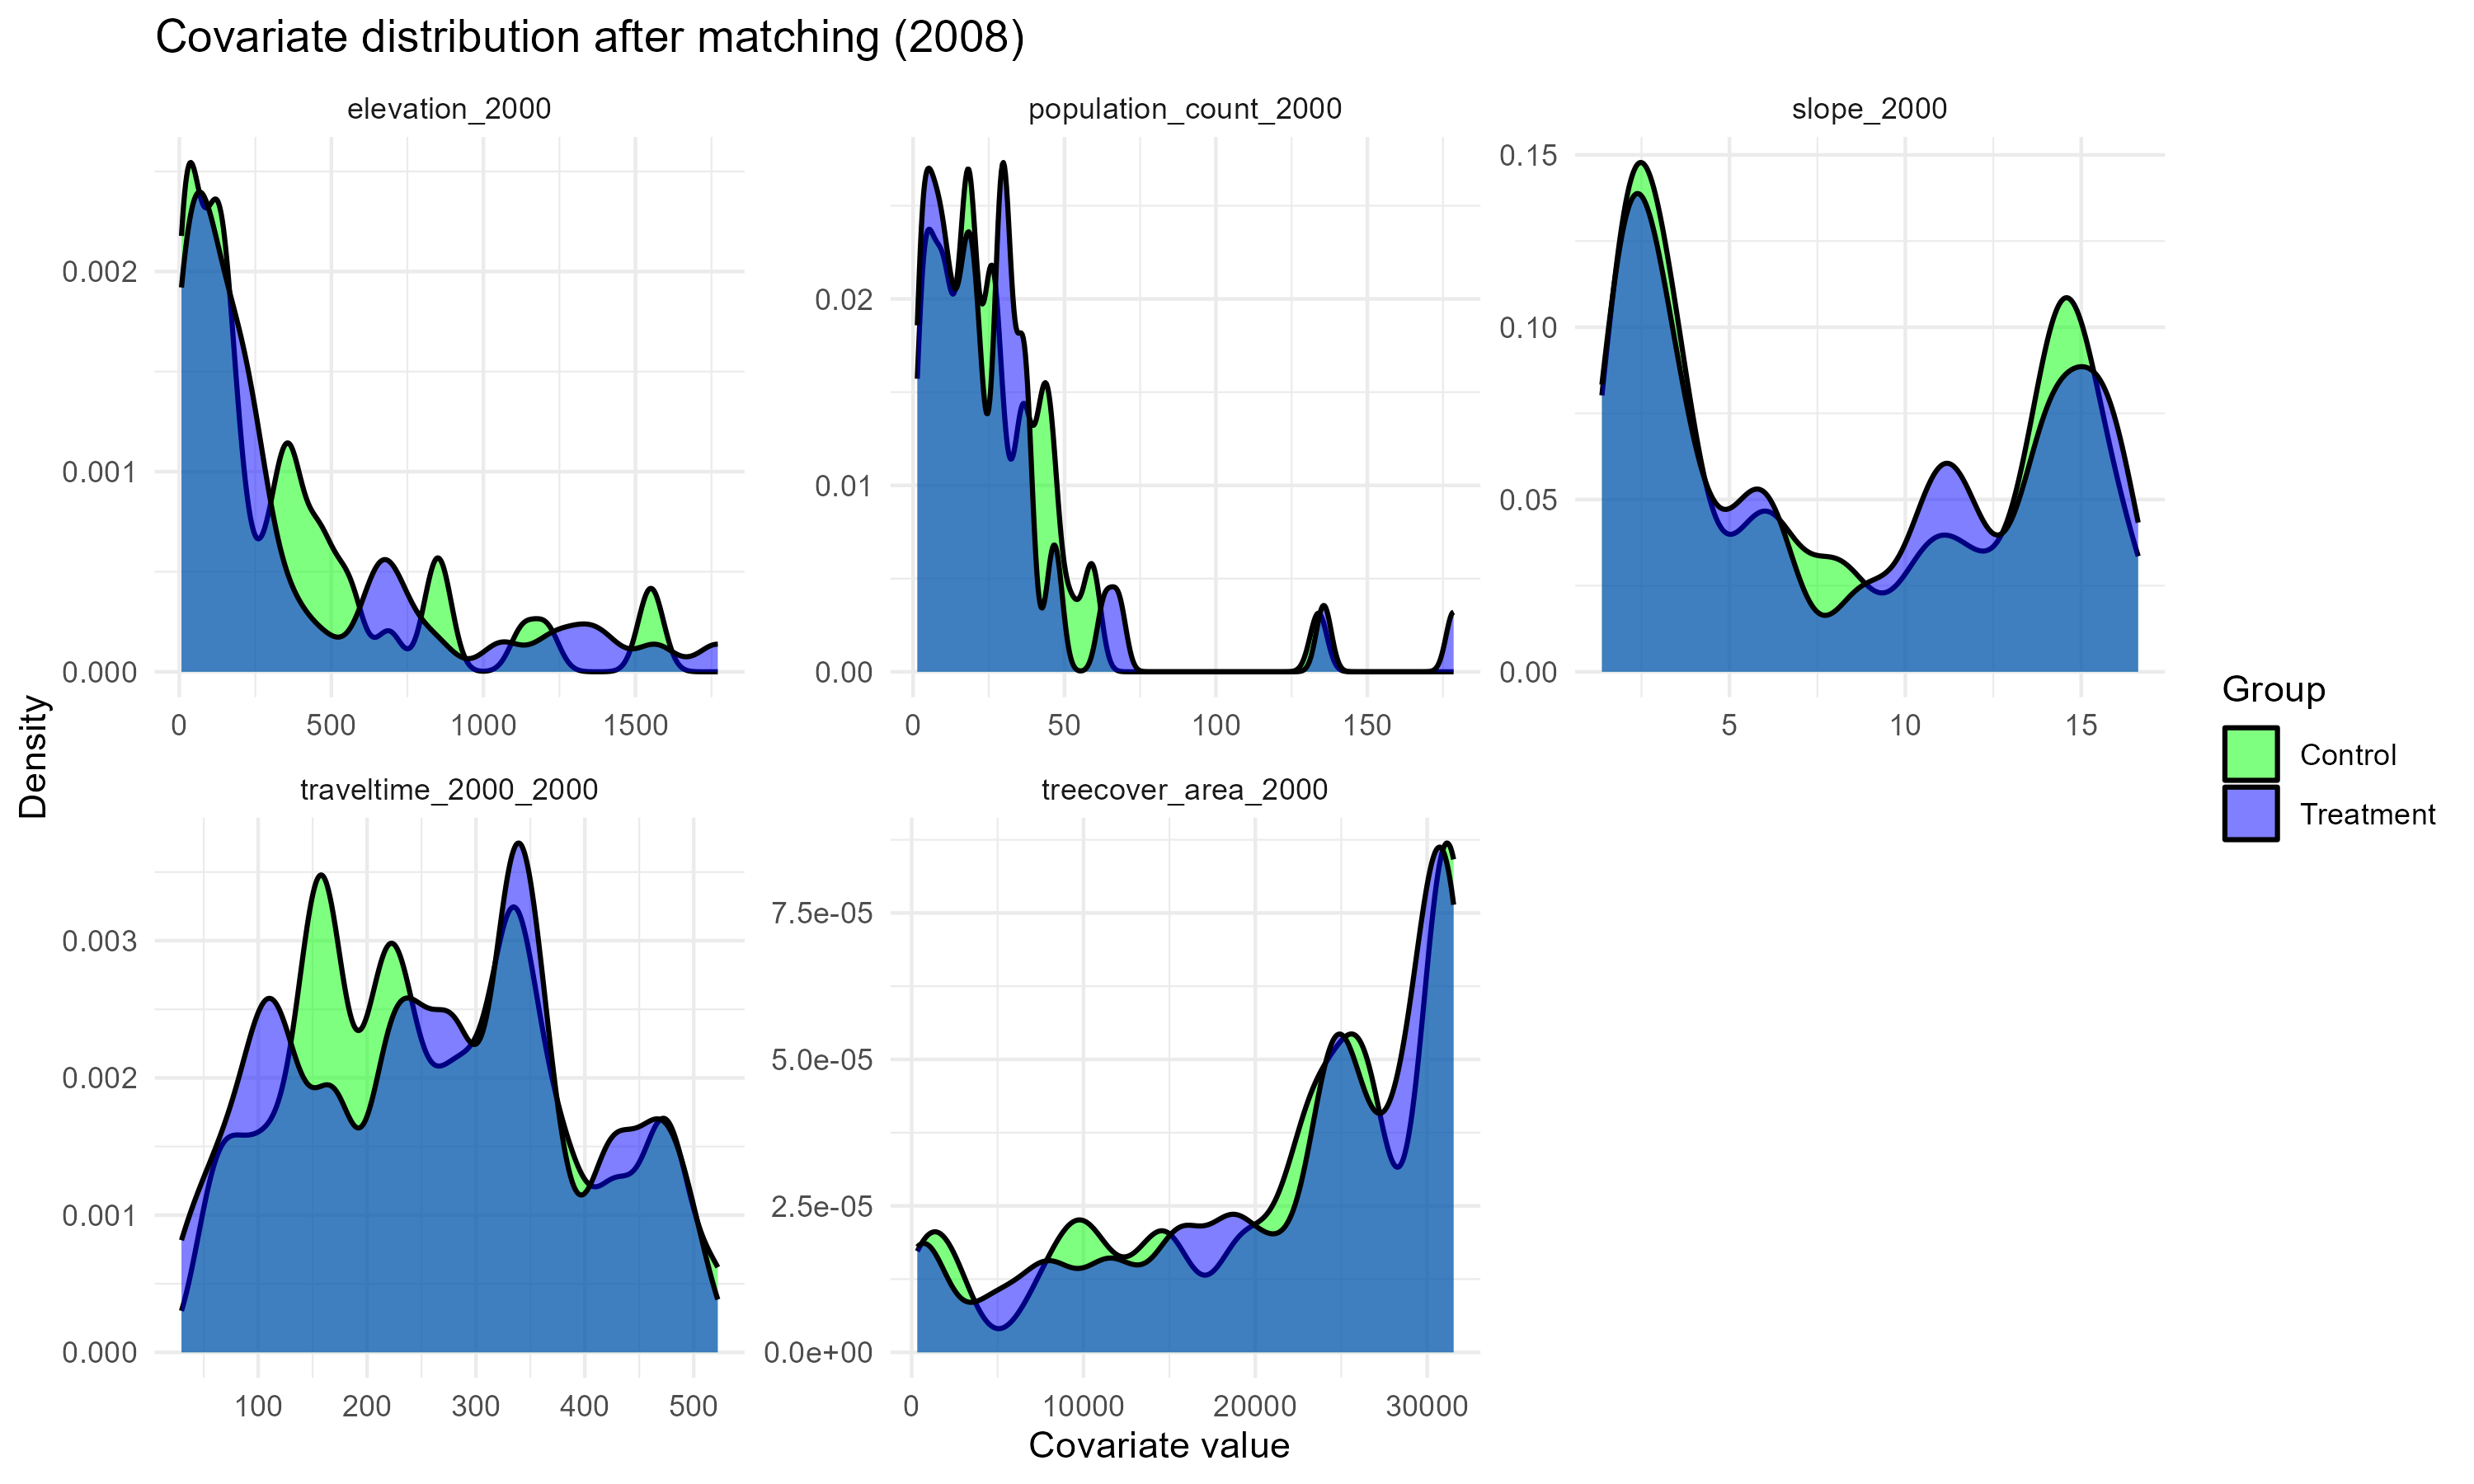
\includegraphics[width=1\linewidth,height=\textheight,keepaspectratio]{images/density_after_2008.png}
\end{block}
\end{column}
\end{columns}
\end{frame}

\begin{frame}{Impact on well-being: Event-study with 2-year bins}
\protect\phantomsection\label{impact-on-well-being-event-study-with-2-year-bins}
\hypertarget{annexe-result-h1}{}

\begin{table}

\caption{\label{tbl-h1-staggered-static}Static treatment effect
estimates on well-being}

\centering{

\centering
\begin{tblr}[         %% tabularray outer open
]                     %% tabularray outer close
{                     %% tabularray inner open
colspec={Q[]Q[]},
hline{2}={1-2}{solid, black, 0.05em},
hline{4}={1-2}{solid, black, 0.05em},
hline{1}={1-2}{solid, black, 0.1em},
hline{11}={1-2}{solid, black, 0.1em},
column{2}={}{halign=c},
column{1}={}{halign=l},
}                     %% tabularray inner close
& did2s (static) \\
treat\_on = 1 & 4.519 \\
& (4.234) \\
Num.Obs. & 4246 \\
R2 & 0.006 \\
R2 Adj. & 0.006 \\
AIC & 41025.8 \\
BIC & 41032.2 \\
RMSE & 30.32 \\
Std.Errors & Corrected Clustered (cluster\_uid) \\
\end{tblr}

}

\end{table}%

\hyperlink{slide-result-h1}{\beamerbutton{$\leftarrow$ Back}}
\end{frame}

\begin{frame}{Impact on inequalities: Event-study with 2-year bins}
\protect\phantomsection\label{impact-on-inequalities-event-study-with-2-year-bins}
\hypertarget{annexe-result_h2}{}

\begin{table}
\centering
\begin{tblr}[         %% tabularray outer open
]                     %% tabularray outer close
{                     %% tabularray inner open
colspec={Q[]Q[]},
hline{2}={1-2}{solid, black, 0.05em},
hline{4}={1-2}{solid, black, 0.05em},
hline{1}={1-2}{solid, black, 0.1em},
hline{11}={1-2}{solid, black, 0.1em},
column{2}={}{halign=c},
column{1}={}{halign=l},
}                     %% tabularray inner close
& did2s (static) \\
treat\_on = 1 & -0.007 \\
& (0.019) \\
Num.Obs. & 4246 \\
R2 & -0.000 \\
R2 Adj. & -0.000 \\
AIC & 7251.5 \\
BIC & 7257.9 \\
RMSE & 0.57 \\
Std.Errors & Corrected Clustered (cluster\_uid) \\
\end{tblr}
\end{table}

\hyperlink{slide-result-h2}{\beamerbutton{$\leftarrow$ Back}}
\end{frame}

\begin{frame}{Robustness Test}
\protect\phantomsection\label{robustness-test}
\begin{itemize}
\tightlist
\item
  \textbf{Distance threshold test of 5 km and 15km}: Proximity to PA has
  no significant effect on wealth
\item
  \textbf{Pseudo-panel analysis}: the results confirm the robustness of
  the conclusions in that environmental and spatial conditions have a
  stronger influence on household living conditions than
  sociodemographic characteristics
\item
  \textbf{Heterogeneity analysis}: The effects are not robust to the
  presence of unobserved bias
\item
  \textbf{Other outcome variables (Child size/weight and infant
  mortality}): No significant effect is found in the estimation
\end{itemize}
\end{frame}




\end{document}
